\chapter{Physical Implementation}

This chapter describes our choosing of physical components, and the implementation of the \gls{pcb}.

\section{Architecture}
The envisioned execution path, shown in figure \ref{fig:PCB_Overview} gives a good idea to what considerations had to be taken when designing the \gls{pcb} and selecting components.

\begin{enumerate}
\item Assembled \vthreek programs are loaded into instruction memory via the EFM32 microcontroller.
\item The \gls{fpga} reads instructions from memory and performs execution.
\item Data ready to be sent to the HDMI output will be stored in a frame buffer, while data aimed for the DACs will be stored in the FPGA's internal block RAM.
\item The output from the \gls{dac}s is displayed on an analogue oscilloscope and the output from the \gls{hdmi} on a raster screen.
\end{enumerate}

The flash memory is a non-volatile storage for the bit file, which will configure the \gls{fpga}, avoiding unnecessary manual configuration for every reboot.

\begin{figure}[h!]
\centering
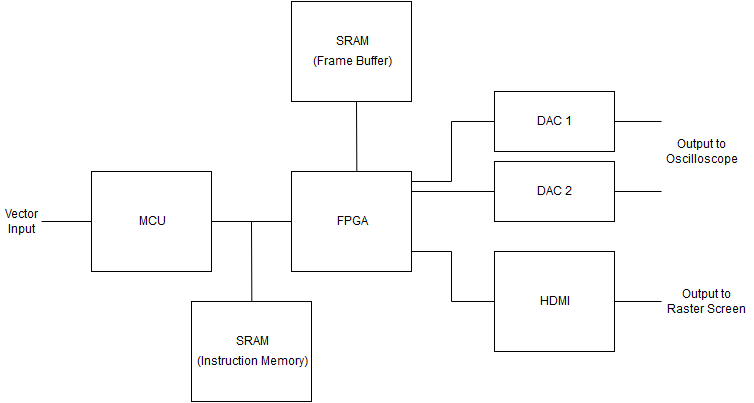
\includegraphics[scale = 0.56]{images/PCB_Overview.png}
\caption{Overview of \gls{pcb} architecture}
\label{fig:PCB_Overview}
\end{figure}

\section{Components}
This section describes the team's choices of components.
All components had to meet the team's technical demands, e.g. number of pins, voltage level support and satisfying outputs.
This information was found by inspecting the various component's datasheets.
Critical components in the design are described in the following subsections.

\subsection{MCU}
The \gls{mcu} is the EFM32GG microcontroller described in Chapter~\ref{ch:mcu}.

\subsection{FPGA}
The \gls{fpga} is a Xilinx XC6SLX45-2CSG324I, with 401 kb block \gls{ram}.
It serves as the main processor in the design, fetching and executing instructions from instruction memory.

A \gls{jtag} header is connected to the \gls{fpga} for good accessibility to \gls{fpga} debugging and programming.
\gls{jtag} is a standard for test logic and connection interface towards integrated circuits \cite{jtag}.

\subsection{SRAM}
Two \gls{sram}s are put on the \gls{pcb}.
One of them works as an instruction memory for the \gls{fpga}, while the other is a dedicated frame buffer for our output signals.
The vector-specific instructions executed in the \gls{fpga} will update the frame buffer, and data from the frame buffer can be read and transferred to the output units.
Both \gls{sram}s has an address space of 512k 16-bit words, which is plenty of space for our design.

\subsection{\gls{dac}s and \gls{bnc}s}
As the purpose of the computer is to output vector graphics on an analogue vector screen, \gls{dac}s are essential.
They will convert digital signals from the \gls{fpga} destined for the output screen, to corresponding analogue signals.

It is important that the \gls{dac}s can output signals fast enough, to minimize flickering.
Therefore, \gls{dac}s that could support clock rates up to 30MHz was chosen by the team.

The \gls{bnc}s connectors receive the analogue signals from the \gls{dac}s and send them to the oscilloscope.
There is one \gls{dac} and one \gls{bnc} for both the x-coordinate and the y-coordinate, or channel 1 and 2, on the oscilloscope.

\subsection{Oscillators}
Two external oscillators are connected to the \gls{mcu}: one low frequency (32,768kHz), and one high frequency (48MHz).
The \gls{mcu} already contains internal RC-oscillators, but external oscillators are much more accurate and stable than the internal ones, which is important for avoiding more sources of errors.
Both crystals or full-fledged oscillators can be used. The team decided to use oscillators.
The reason behind this choice was that an oscillator is one fully built component with all the necessary circuitry inside, and the datasheet clearly specified how it should be connected.
Crystals, on the other hand, requires load capacitors, whose values weren't properly specified.
Another reason is that our \gls{fpga} explicitly needed an external oscillator, as a crystal is incompatible with the design.
Hence, the team chose oscillators for both the \gls{fpga} and \gls{mcu} for simplicity.
A 100MHz oscillator was chosen for the \gls{fpga}, to make sure too low frequency wouldn't be an issue.

\subsection{Buses}
The system utilizes one parallel bus (\gls{ebi}), and one serial bus (\gls{spi}).
The \gls{mcu} acts as bus master for both of them, since it supplies the bus technologies.

\subsubsection{\gls{ebi}}
The \gls{fpga}, \gls{mcu} and \gls{sram} are all connected via the \gls{ebi} bus.
These connections are made properly by using the specified \gls{ebi}-pins on the \gls{mcu} \cite[sec. 4.1]{efm32-datasheet}.
The \gls{ebi} bus is a parallel bus that allows high-speed communication to the \gls{sram}, and the following bus lines are included in our implementation:

\begin{itemize}
\item 23 Address bits. More than initially needed, since SRAM have 19-bit addresses, but this is increased for good measure.
\item 16 Data bits, as our \gls{sram} consisted of 16-bit words.
\item 2 Chip select bits, one for the \gls{fpga} and one for the \gls{sram}.
\item 1 Write enable bit, active low.
\item 1 Read enable bit, active low.
\end{itemize}

\subsubsection{\gls{spi}}
The \gls{spi} serves as a three-way communication between the \gls{mcu}, \gls{fpga} and the flash memory.
It's main purpose is to make the \gls{fpga} be configured from a bit-file stored in the flash memory.
As opposed to the \gls{ebi} bus, \gls{spi} is a serial bus, transferring one bit of data at a time.

\subsection{Buttons and \gls{led}s}
All buttons include a resistor for current limitation (to avoid short circuits) and pull-up (to avoid logical floating state).
The exception is the button connected to the \gls{mcu}, where the pin has an internal pull-up.
All \gls{led}s also include a current limiting resistor.
Ohms law was used to calculate the required resistance \cite{ohm}.

\gls{led}s are handy for giving an indication that something is turned on.
For instance, the design includes a \gls{led} which will light up when the \gls{fpga} is configured.
Buttons are used for triggering events, e.g. reset.

\subsection{Power Supply}
The \gls{pcb} will receive power from a micro-\gls{usb} connector.
A voltage level of 5V is sufficient, since no components require more than this.
However, plenty of components require less than 5V, most of them 3.3V.
To lower the voltage to a specific level, voltage regulators are used.
Power is discussed in more detail in section \ref{Power}.

\subsection{Decoupling Capacitors}
Several major components requires decoupling, e.g. the \gls{mcu}, \gls{fpga}, voltage regulators and \gls{dac}s.
Decoupling means connecting power supplies through a capacitor network to ground, where power moving to ground can be temporarily stored.
This is necessary as it sometimes occurs situations where there is suddenly high need for power.
The power supply alone will not always be able to support these 'bursts'.
With a capacitor decoupling network, the component can pull extra power from the capacitors added to the regular power supply.

\section{\gls{pcb} Design}
The architecture is realized on a \gls{pcb} designed using Altium Designer 15.1.
Having never used this program before, the group had to overcome challenges and difficulties related to not only learning new software, but also learning concepts of creating a \gls{pcb} from scratch.

\subsection{Schematics}
The entire logic of the \gls{pcb} are designed with schematics.
Altium has been used to map the components together, pin by pin.
Making the right connections and pin mappings is the only thing that matters in the schematics.
That means there was no focus on physical \gls{pcb}-specific things, e.g. routing and component placement.

When the schematics were completed, the team moved on to design the physical \gls{pcb}.
The complete schematics are in appendix \ref{app:schematics}.

\subsection{Component Placement}
Components are placed on the \gls{pcb}, so that they are in close range of all other components they have to connect with.
This is desirable for shortening the routing, which is positive in terms of mitigating signal delay and maintaining signal integrity.

The \gls{fpga}, \gls{sram}s and \gls{mcu} are the most important components with a lot of different connections, and are therefore placed central on the \gls{pcb}.
\gls{io} components, e.g. controller buttons, \gls{usb}, \gls{hdmi} and \gls{bnc} receptacles, are placed along the edge, since these are typically connected to few other components.
It would also be annoying to connect external peripheral plugs to sockets in the middle of the \gls{pcb}.

All decoupling capacitors involved in the decoupling network for a certain component, are placed in close proximity to that component.
This minimizes the risk that the component won't get the extra power supply it needs during bursts.

All capacitors and resistors are placed on the bottom layer of the \gls{pcb} to save space on an already crowded top layer.

\subsubsection{Component Footprints}
A component footprint is how the trace of a component looks like on the \gls{pcb}.
Many fitting default footprints are already in the standard Altium library, so no customization was needed here.
However, the capacitors and resistors have by default, gigantic footprints, which was not desirable, since the \gls{pcb} needed a large amount of them.
Alternative footprints have been found using the Altium Vault, which the team used to change the capacitor footprint to much smaller one.

\subsection{Layers}
The \gls{pcb} consist of six signal layers: Top layer, bottom layer and four in between.
Two power layers are utilized: \(V_{CC}\) and ground.
Between every signal and power layer, a dielectric layer are added to ensure proper isolation between these conducting layers, such that they won't interfere with each other.

An overlay is added to both the top and bottom layers.
Each overlay contains silk-screen for marking components, thus making it easier to navigate the \gls{pcb}.

The complete layer stack is shown in Figure \ref{fig:Layers}

\begin{figure}[h!]
\centering
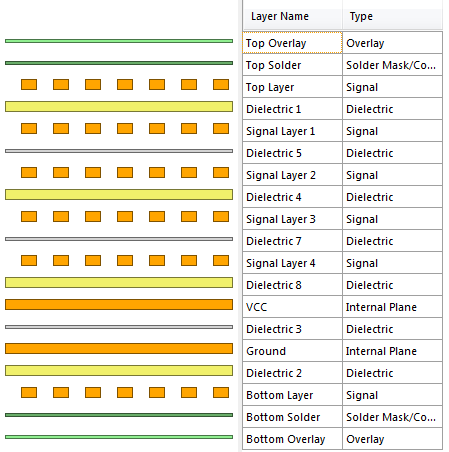
\includegraphics[scale = 0.8]{images/Layers.png}
\caption{Layer Stack}
\label{fig:Layers}
\end{figure}

\subsubsection{Power and ground}
\label{Power}
The \gls{pcb} is designed with three power domains, each with their corresponding voltage regulator: 3.3V, 1.2V and a 5V reserved for analogue signals.
Most components are supplied by the 3.3V regulator, except for some internal parts of the \gls{fpga} that requires 1.2V.

Since 3.3V is used by most components, and since only a few connectors requires 1.2V, a dedicated power plane for 3.3V is added.
A dedicated ground plane is also added.
This significantly simplifies routing, since everything connected to 3.3V or ground can go straight to a multi-layer via, connected to the corresponding plane.
The 1.2V traces has to be routed through all the connectors like any other signal.

\subsubsection{Split planes}
The story of analogue 5V is a little different.
The reason for an analogue 5V is to minimize noise from digital signals.
The analogue components are sensitive to noise from the digital circuitry, and it is crucial to have as little noise as possible on the signal going to the oscilloscope.
To minimize noise, the analogue and digital circuitry has been separated.
Analogue components can not use the same voltage supply as the digital ones, and the same matters for ground.

The solution is splitting of the power and ground plane, shown in Figure \ref{fig:Split planes}.
\begin{itemize}
\item 5AV: Analogue 5V for components on the analogue plane.
The reason for 5V is based on insecurity about how much voltage the oscilloscope requires to properly display vector graphics from the program.
3.3V can be too low, so 5V has been chosen.
A high signal voltage can also potentially help reduce noise. //TODO: What does this mean?
\item AGND: Analogue components are connected to this ground instead of digital ground.
This is to stop the analogue signal from getting disturbed by the digital signals on the ground plane.
\item 3.3V: Digital voltage for digital components.
\item GND: Digital ground.
\end{itemize}

All analogue components are placed in the analogue plane, and the opposite with digital components.
The exception is the \gls{dac}s, which acts as a bridge between the digital part and the analogue part.
These are placed on the actual split, with the affected pins on the correct side.

To lower digital noise that could potentially accumulate on the analog ground plane, a diode is placed between the two ground planes.
The diode lets the current flow from the analogue ground to the digital ground, but not vice versa.

\begin{figure}[h!]
\centering
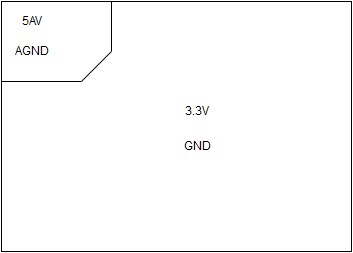
\includegraphics[scale = 0.6]{images/Split_planes.png}
\caption{Split between analogue and digital planes. The separating line is a solid, non-conducting material}
\label{fig:Split planes}
\end{figure}

\section{Routing}
The components has been physically connected according to the schematics, by routing.
Some connections have been manually routed, but Altium's auto router have routed most parts, to speed up the process.

\subsection{Design Rules}
Before routing, necessary rules had to be defined to make sure the \gls{pcb} was routed properly.
The following listing explains the most important rules for the design.
\begin{itemize}
\item Clearance: 0.1mm.
\newline
Minimum clearance between different traces
\item Width: 0.127mm, Power Width 0.203mm.
\newline
Minimum width for traces.
Power traces have bigger minimum widths, than signal traces.
\item Via Diameter: 0.4mm, Via Hole Size: 0.2mm
\newline
Minimum diameter and hole size for multi-layer vias.
\item Short-circuits and net antennas not allowed
\end{itemize}

The rules are set like this to make sure there wouldn't be any interference between traces, while the traces are still wide enough to not get damaged by the signal itself.
Power traces are wider to make sure they can handle the voltage.
Net antennas are traces that lead to dead-ends.
Dead-ends could harm the design, since they can work as unwanted signal receivers from nearby sources.

\subsubsection{Design Rule Check}
Altium has it's own tool for testing how many design rule violations our current design created, called Design Rule Check.
It displays the amount of errors occurred from each type, and the coordinates on the \gls{pcb} for every error.
It has been frequently used during routing.

\section{Fault Handling}
The team were all inexperienced with \gls{pcb} design and often uncertain if actions or decisions could cause problems down the line.
The top priority has been to make something that worked properly.
A failing component is deemed probable, and forgetting something is guaranteed to happen, considering the vast amount of factors involved.
Hence, the team have decided that having back-up features on the \gls{pcb} is critical.

\subsection{Headers}
The primary strategy of handling faults is redundancy, mostly in the form of header pins.
The final amount of headers have ended up at 34, including the \gls{jtag} and the ARM programming header.
Using this large amount of headers have made it possible to measure most signals with a multimeter and verify them.
The team got this idea from reading the Demolicious report \cite{demolicious-report}, from last years computer design project.

Most headers are placed between components.
If wrong connections exist, or a connection don't work, the connection can most likely be corrected by connecting wires.

\begin{figure}[h!]
\centering
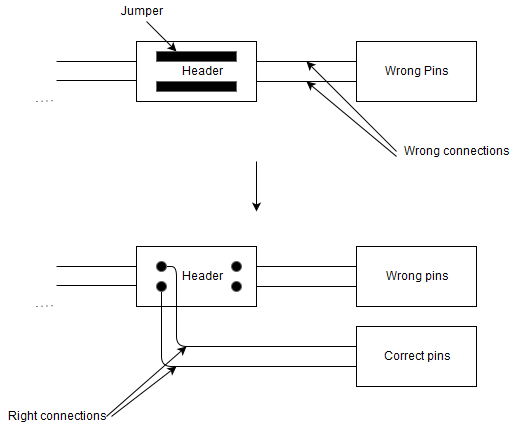
\includegraphics[scale = 0.57]{images/Header_fix.png}
\caption{Example Header fix}
\label{fig:Header fix}
\end{figure}

Headers are also useful as switches.
By manually connecting header pins with jumpers, certain parts of the \gls{pcb} can be activated and deactivated.
This will be useful when focusing on lesser parts of the circuit.
For instance, 3-pin headers are used to manually turn on and off different voltage levels.
Power can also be delivered to the components directly through the headers, if any issue with the power supply should occur.

\subsection{DACs}
Even though separate \gls{dac}s for outputting analog voltage out to the \gls{bnc} plug are included, there is still a risk that the group won't get them to work.
A back-up solution by connecting the internal \gls{dac}s in the \gls{mcu} to the \gls{bnc}s is implemented.
One 2x2 header for each \gls{bnc} input is used to manually control whether the main \gls{dac}s or the \gls{mcu} \gls{dac}s will to be used.
This process is shown in figure \ref{fig:DAC headers}.
There's one header each for the X and the Y signal to the oscilloscope.

\begin{figure}[h!]
\centering
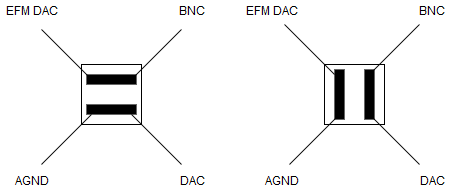
\includegraphics[scale = 0.6]{images/DAC_headers.png}
\caption{Left: Jumpers connecting \gls{mcu} \gls{dac} to \gls{bnc} and normal \gls{dac} to ground. Right: The opposite}
\label{fig:DAC headers}
\end{figure}
